% Options for packages loaded elsewhere
\PassOptionsToPackage{unicode}{hyperref}
\PassOptionsToPackage{hyphens}{url}
%
\documentclass[
]{article}
\usepackage{amsmath,amssymb}
\usepackage{iftex}
\ifPDFTeX
  \usepackage[T1]{fontenc}
  \usepackage[utf8]{inputenc}
  \usepackage{textcomp} % provide euro and other symbols
\else % if luatex or xetex
  \usepackage{unicode-math} % this also loads fontspec
  \defaultfontfeatures{Scale=MatchLowercase}
  \defaultfontfeatures[\rmfamily]{Ligatures=TeX,Scale=1}
\fi
\usepackage{lmodern}
\ifPDFTeX\else
  % xetex/luatex font selection
\fi
% Use upquote if available, for straight quotes in verbatim environments
\IfFileExists{upquote.sty}{\usepackage{upquote}}{}
\IfFileExists{microtype.sty}{% use microtype if available
  \usepackage[]{microtype}
  \UseMicrotypeSet[protrusion]{basicmath} % disable protrusion for tt fonts
}{}
\makeatletter
\@ifundefined{KOMAClassName}{% if non-KOMA class
  \IfFileExists{parskip.sty}{%
    \usepackage{parskip}
  }{% else
    \setlength{\parindent}{0pt}
    \setlength{\parskip}{6pt plus 2pt minus 1pt}}
}{% if KOMA class
  \KOMAoptions{parskip=half}}
\makeatother
\usepackage{xcolor}
\usepackage[margin=1in]{geometry}
\usepackage{color}
\usepackage{fancyvrb}
\newcommand{\VerbBar}{|}
\newcommand{\VERB}{\Verb[commandchars=\\\{\}]}
\DefineVerbatimEnvironment{Highlighting}{Verbatim}{commandchars=\\\{\}}
% Add ',fontsize=\small' for more characters per line
\usepackage{framed}
\definecolor{shadecolor}{RGB}{248,248,248}
\newenvironment{Shaded}{\begin{snugshade}}{\end{snugshade}}
\newcommand{\AlertTok}[1]{\textcolor[rgb]{0.94,0.16,0.16}{#1}}
\newcommand{\AnnotationTok}[1]{\textcolor[rgb]{0.56,0.35,0.01}{\textbf{\textit{#1}}}}
\newcommand{\AttributeTok}[1]{\textcolor[rgb]{0.13,0.29,0.53}{#1}}
\newcommand{\BaseNTok}[1]{\textcolor[rgb]{0.00,0.00,0.81}{#1}}
\newcommand{\BuiltInTok}[1]{#1}
\newcommand{\CharTok}[1]{\textcolor[rgb]{0.31,0.60,0.02}{#1}}
\newcommand{\CommentTok}[1]{\textcolor[rgb]{0.56,0.35,0.01}{\textit{#1}}}
\newcommand{\CommentVarTok}[1]{\textcolor[rgb]{0.56,0.35,0.01}{\textbf{\textit{#1}}}}
\newcommand{\ConstantTok}[1]{\textcolor[rgb]{0.56,0.35,0.01}{#1}}
\newcommand{\ControlFlowTok}[1]{\textcolor[rgb]{0.13,0.29,0.53}{\textbf{#1}}}
\newcommand{\DataTypeTok}[1]{\textcolor[rgb]{0.13,0.29,0.53}{#1}}
\newcommand{\DecValTok}[1]{\textcolor[rgb]{0.00,0.00,0.81}{#1}}
\newcommand{\DocumentationTok}[1]{\textcolor[rgb]{0.56,0.35,0.01}{\textbf{\textit{#1}}}}
\newcommand{\ErrorTok}[1]{\textcolor[rgb]{0.64,0.00,0.00}{\textbf{#1}}}
\newcommand{\ExtensionTok}[1]{#1}
\newcommand{\FloatTok}[1]{\textcolor[rgb]{0.00,0.00,0.81}{#1}}
\newcommand{\FunctionTok}[1]{\textcolor[rgb]{0.13,0.29,0.53}{\textbf{#1}}}
\newcommand{\ImportTok}[1]{#1}
\newcommand{\InformationTok}[1]{\textcolor[rgb]{0.56,0.35,0.01}{\textbf{\textit{#1}}}}
\newcommand{\KeywordTok}[1]{\textcolor[rgb]{0.13,0.29,0.53}{\textbf{#1}}}
\newcommand{\NormalTok}[1]{#1}
\newcommand{\OperatorTok}[1]{\textcolor[rgb]{0.81,0.36,0.00}{\textbf{#1}}}
\newcommand{\OtherTok}[1]{\textcolor[rgb]{0.56,0.35,0.01}{#1}}
\newcommand{\PreprocessorTok}[1]{\textcolor[rgb]{0.56,0.35,0.01}{\textit{#1}}}
\newcommand{\RegionMarkerTok}[1]{#1}
\newcommand{\SpecialCharTok}[1]{\textcolor[rgb]{0.81,0.36,0.00}{\textbf{#1}}}
\newcommand{\SpecialStringTok}[1]{\textcolor[rgb]{0.31,0.60,0.02}{#1}}
\newcommand{\StringTok}[1]{\textcolor[rgb]{0.31,0.60,0.02}{#1}}
\newcommand{\VariableTok}[1]{\textcolor[rgb]{0.00,0.00,0.00}{#1}}
\newcommand{\VerbatimStringTok}[1]{\textcolor[rgb]{0.31,0.60,0.02}{#1}}
\newcommand{\WarningTok}[1]{\textcolor[rgb]{0.56,0.35,0.01}{\textbf{\textit{#1}}}}
\usepackage{graphicx}
\makeatletter
\def\maxwidth{\ifdim\Gin@nat@width>\linewidth\linewidth\else\Gin@nat@width\fi}
\def\maxheight{\ifdim\Gin@nat@height>\textheight\textheight\else\Gin@nat@height\fi}
\makeatother
% Scale images if necessary, so that they will not overflow the page
% margins by default, and it is still possible to overwrite the defaults
% using explicit options in \includegraphics[width, height, ...]{}
\setkeys{Gin}{width=\maxwidth,height=\maxheight,keepaspectratio}
% Set default figure placement to htbp
\makeatletter
\def\fps@figure{htbp}
\makeatother
\ifLuaTeX
  \usepackage{luacolor}
  \usepackage[soul]{lua-ul}
\else
  \usepackage{soul}
\fi
\setlength{\emergencystretch}{3em} % prevent overfull lines
\providecommand{\tightlist}{%
  \setlength{\itemsep}{0pt}\setlength{\parskip}{0pt}}
\setcounter{secnumdepth}{-\maxdimen} % remove section numbering
\ifLuaTeX
  \usepackage{selnolig}  % disable illegal ligatures
\fi
\usepackage{bookmark}
\IfFileExists{xurl.sty}{\usepackage{xurl}}{} % add URL line breaks if available
\urlstyle{same}
\hypersetup{
  pdftitle={CACCS: Secuencia de taller de RStudio -- Parte 1},
  pdfauthor={Rashid C.J. Marcano Rivera},
  hidelinks,
  pdfcreator={LaTeX via pandoc}}

\title{CACCS: Secuencia de taller de RStudio -- Parte 1}
\author{Rashid C.J. Marcano Rivera}
\date{5 de feb.º de 2025}

\begin{document}
\maketitle

{
\setcounter{tocdepth}{2}
\tableofcontents
}
\textbf{Introducción a la computación estadística en R}

Este taller está basado en notas de Paul Thibodeau y revisiones de
profesores del departamento de psicología de BYU
\href{https://fhssrsc.byu.edu/r-workshop}{(vea esa versión aquí)}.
Adaptado al español y usando ejemplos del libro de Rafael Irizarry
\href{https://leanpub.com/dslibro}{disponible aquí}. Ha sido revisado de
la primera versión de este taller, brindado en el Centro Académico de
Cómputos de Ciencias Sociales en octubre de 2024.

\emph{Si aún no has instalado R, está disponible
\href{http://cran.us.r-project.org/}{aquí}. Acto seguido,
\href{https://posit.co/download/rstudio-desktop/}{baja RStudio}. Puedes
también ir a la nube \href{https://posit.cloud/}{en Posit Cloud}.}

\section{Sobre aprender R}\label{sobre-aprender-r}

R es un lenguaje creado por estadísticos como ambiente interactivo para
análisis de datos. En R pueden guardar su trabajo como una secuencia de
comandos, conocida como un \emph{script}, que se pueden ejecutar
fácilmente en cualquier momento, con portabilidad. Estos \emph{scripts}
sirven como un registro del análisis que realizaron, una característica
clave que facilita el trabajo \ul{\textbf{\emph{reproducible}}}. Si bien
es un programa poderoso y flexible, es ciertamente más complicado que
programados como el que puedan encontrar en SPSS o STATA, donde pueden
señalar con el ratón una opción y ejecutarla. Por otro lado, R es
gratuito y de código abierto. En adición es modular y las
funcionalidades añadidas complementariamente por terceros también son
gratuitos, incluyendo acceso temprano a los métodos y herramientas más
recientes que se desarrollan para una amplia variedad de disciplinas,
incluyendo la economía, ciencias políticas, sociología, planificación,
ecología, geografía o la biología molecular, entre otros.

Mi idea tras esta secuencia de talleres sobre R es brindar una
introducción para que puedan interactuar con R tal que los sentimientos
de frustración o ansiedad que puedan surgir al trabajar con este
lenguaje al usarlo en variedad de circunstancias. Este taller presume en
general ciertos conocimientos básicos en estadística, pero abundará en
cada parte que se trabaje aunque sea algo como la motivación para las
funciones que ejecutaremos. So no tienen experiencia en programación
computacional, es posible que partes de este taller resulten confusas o
no tengan mucho sentido. Recomiendo que aún así traten de entender lo
que puedan, y luego al volver a este taller periódicamente al repasar el
contenido, vayan comprendiendo (o trayendo preguntas que no se
resuelvan) el material.

Es importante que sepan que la habilidad más útil de antemano es la de
saber adónde ir cuando se atasquen. R ayuda bastante en esto. La consola
de R, al escribir y ejecutar comandos, brinda retroalimentación
inmediata. Hagan uso de esto de manera liberal mientras trabajan el
taller, haciendo pequeñas modificaciones a los ejemplos que brinde,
hasta que sientan que entienden qué está ocurriendo.

De una vez, cabe señalar que la consola brinda acceso a la función de
buscar ayuda interna. Casi todas las funciones (y muchos de los datos
pre-almacenados) tienen archivos que les acompañan describiendo qué son
las funciones, y cómo usarlas. Pueden acceder a esta información
escribiendo \texttt{help(función)} (o \texttt{?función}), sustituyendo
«función» por el nombre de la función que quieras conocer. Es importante
leer estos archivos detenidamente la primera vez que te encuentres con
una función, pero \emph{también} (posiblemente más) importante es
consultarlos con frecuencia. Si tienes una idea de qué quieres hacer,
pero no sabes ni recuerdas la función exacta para esto, puedes buscar en
los archivos por el término usando doble signo de interrogación
(\texttt{??regression}).

Hay mucha información adicional en internet. Es difícil buscar en Google
por R, ya que es una letra, pero sí se puede encontrar mucho sobre
funcionalidades. Para búsqueda más certera se puede ir a
\href{http://stackoverflow.com/}{StackOverflow}, y buscar el tag de R
(\texttt{{[}R{]}}) junto a tu pregunta o error. Relacionado está el
\href{http://stats.stackexchange.com/}{StackExchange de estadísticas},
que es como Stack Overflow pero enfocado en la madeja estadística.

Finalmente, antes de empezar, quiero hablar sobre errores. Tanto novatos
como expertos encontrarán errores en su código de R. De suceder, al ir
ejecutando un \emph{script} o trabajo, cesará el proceso y saldrá
impreso un mensaje de error en la consola. Esto puede ser frustrante, en
especial al estar iniciando el aprendizaje, pues el error ocurre a
menudo muy adentro de las especificidades de una función, y el mensaje
de error no guarda relación con lo que el usuario quería hacer. Un error
a evitar al empezar a aprender R es que el error es un disparate
incomprensible, y resignarse a la frustración y desánimo. Resistan ese
impulso; si bien el mensaje no será de inicio informativo, está diseñado
para transmitir cierta información con claridad, y entender esa
información es clave para resolver el problema (o cambiar de
estrategias).

Esta es una secuencia de tres semanas, y en esta lección arrancaremos
con lo básico de R, RStudio, y tenemos la meta hoy de que al culminar
las primeras dos horas de esta secuencia podamos:

\begin{enumerate}
\def\labelenumi{\arabic{enumi}.}
\item
  Entender la lógica de RStudio.
\item
  Importar, crear, leer y manipular datos y objetos.
\item
  Inicios de la visualización y análisis descriptivo.
\end{enumerate}

Durante las próximas cuatro semanas expandiremos sobre esta base, y
profundizaremos el miércoles 12 de febrero en visualización avanzada,
para datos transversales, series de tiempo, y datos censales así como de
otros acercamientos, usando herramientas de \texttt{ggplot2} y
\texttt{sf}. Luego, la tercera semana, del 19 de febrero, entraremos más
en \emph{wrangling} de datos, así como en la inferencia estadística, con
introducciones en R sobre modelos lineales, jerárquicos y
longitudinales, así como de los distintos métodos de verificación de
presunciones de modelo. Finalmente, en la cuarta semana, del 26 de
febrero, trabajaremos en la medida de lo posible, con análisis o ciencia
de redes. Si bien hay mucho más que se puede hacer con R
(e.g.~\emph{machine learning,} extracción de datos de la web,
procesamiento de cadenas y minería de textos, interacción con Git,
trabajos en Unix, o nuevos desarrollos en Quarto), la idea es iniciar la
travesía en R, y señalar a dónde pueden buscar ahondar.

\subsection{Usando RStudio (y presentando por encima,
RMarkdown)}\label{usando-rstudio-y-presentando-por-encima-rmarkdown}

¿Cómo difieren R y RStudio? RStudio es una interfaz que yace encima del
programa base R. Es además \ul{\textbf{mucho}} más amigable y llevadera
que R.

\begin{figure}
\centering
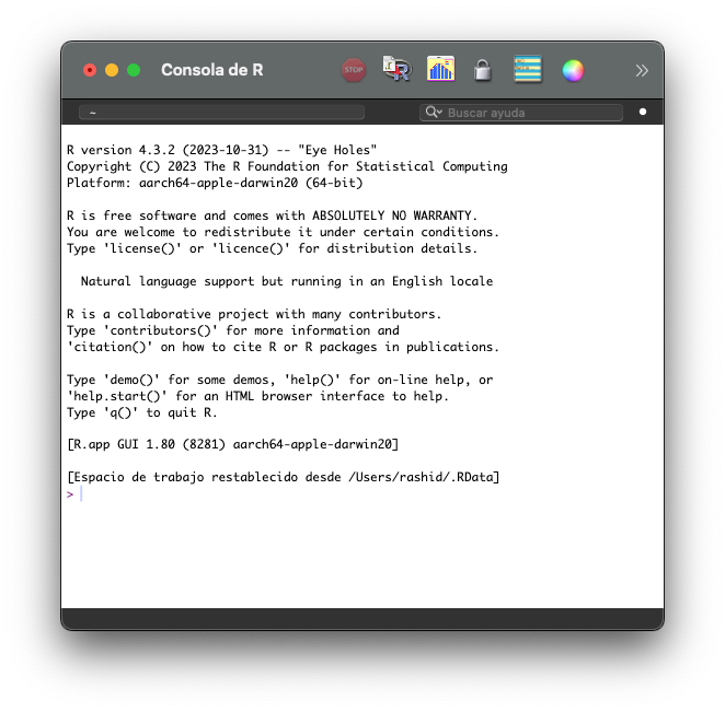
\includegraphics{R.png}
\caption{Consola R: ejecuta comandos a la medida que se escriben.}
\end{figure}

R, por su cuenta es una consola sencilla donde teclean y corren código.

\begin{figure}
\centering
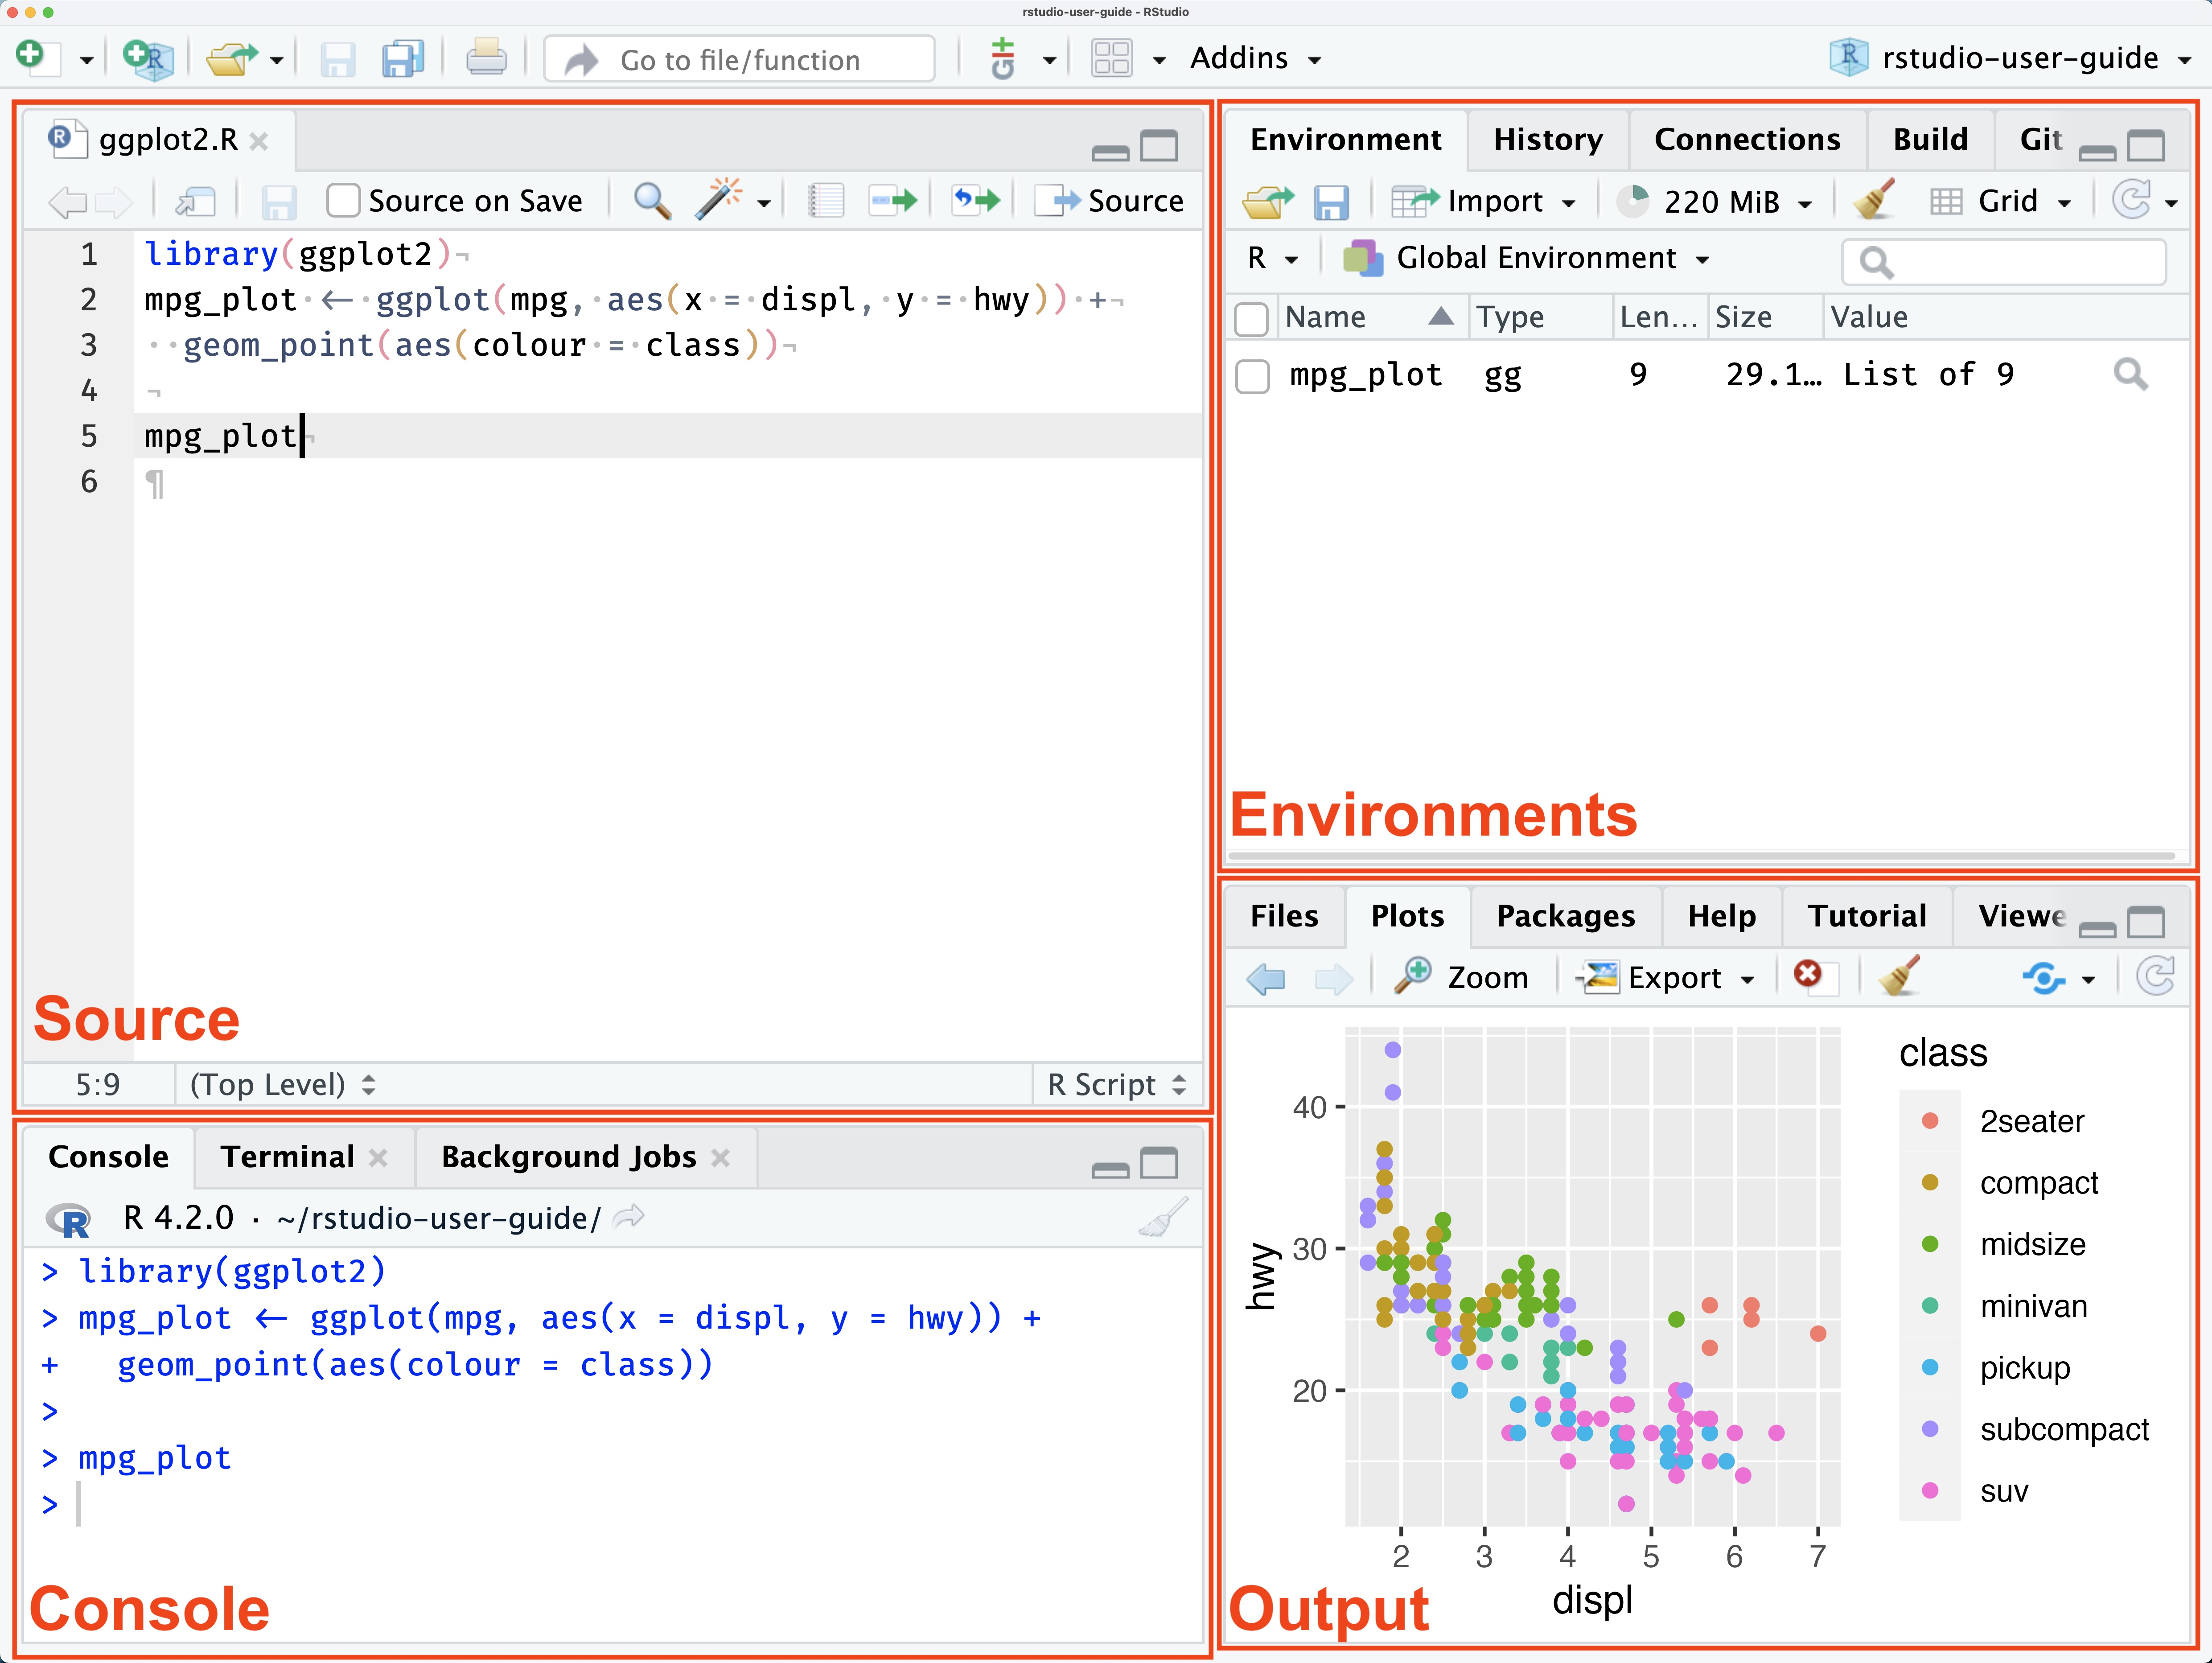
\includegraphics{RStudioPanes.jpeg}
\caption{RStudio con varios paneles, incluyendo la consola inicial de R
(abajo a la izquierda).}
\end{figure}

RStudio tiene la \emph{Consola} como panel, pero tiene otros paneles en
adición que nos ayudan a ubicarnos, como \emph{Environment} (Ambiente) -
para que vean los objetos (conjuntos de datos y variables, o funciones)
que hayan guardado o creado a través de la sesión \emph{-} el de
\emph{Output} (Salida) - donde pueden ver sus archivos en el directorio,
sus gráficos, acceder los paquetes y buscar ayuda - y \emph{Source}
(Fuente), donde pueden crear y editar tanto archivos o \emph{scripts} de
R, como de Markdown,
\href{https://quarto.org/docs/get-started/hello/rstudio.html}{Quarto} y
\href{https://shiny.posit.co/r/getstarted/shiny-basics/lesson1/index.html}{Shiny}
(para dashboards), entre otros formatos.

Estos paneles (y otras configuraciones) son editables, como el caso del
R que manejo en mi Mac:

\begin{figure}
\centering
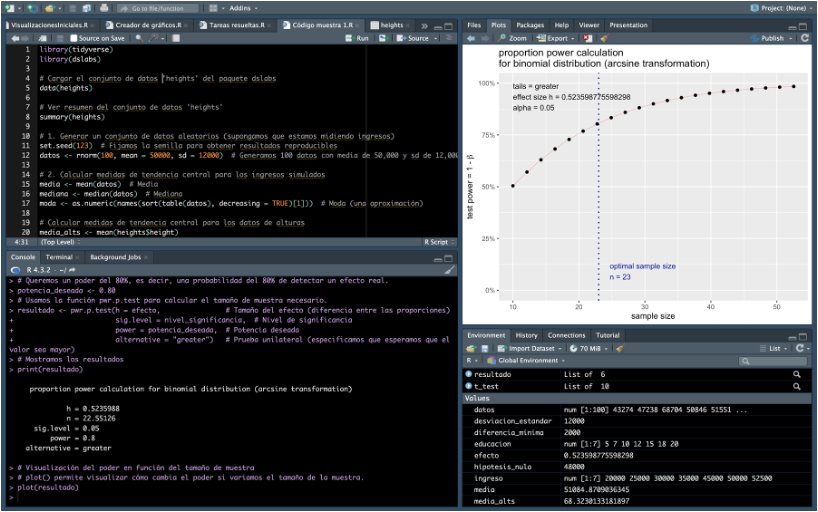
\includegraphics{RStudio.png}
\caption{Otra forma posible de configuración.}
\end{figure}

A grosso modo, RMarkdown es un tipo de documento que permite la
escritura de texto regular junto a secciones o pedazos de R. Esto es
útil para explicar por ejemplo tu código, seguido por el código mismo
para uso regular. También es útil porque Markdown se puede exportar como
una página html así como un PDF, lo cual es útil para compartirlo fuera
del esquema de R. Si les interesara más sobre RMarkdown, visiten esta
\href{https://rmarkdown.rstudio.com/lesson-1.html}{página}.

\section{Interacción con la consola de
R}\label{interacciuxf3n-con-la-consola-de-r}

\begin{Shaded}
\begin{Highlighting}[]
\CommentTok{\#install.packages("dslabs","wooldridge","tidyverse") \#Si ya están instalados, comenten con \textquotesingle{}\#\textquotesingle{} para desactivar esta línea}
\end{Highlighting}
\end{Shaded}

En la forma básica, R es una calculadora para cómputos básicos. Escribe
en R (o en un trozo o \textbf{chunk} en RMarkdown) y el resultado saldrá
en la consola al ejecutar o correrlo. Un \textbf{chunk} se designa en
Markdown con triple ` al inicio y fin, así como \{r título de sección\}.
Ahí va el código. Hoy nos enfocaremos en R, pero esta presentación se
hizo en RMarkdown. Pueden correr líneas de su secuencia de códigos al
usar Command+Return en Mac, o Control+Enter en la PC. También hay un
botón para correr líneas o secciones enteras, así como el \emph{script}
entero.

\begin{Shaded}
\begin{Highlighting}[]
\DecValTok{1} \SpecialCharTok{+} \DecValTok{2}
\end{Highlighting}
\end{Shaded}

\begin{verbatim}
## [1] 3
\end{verbatim}

\begin{Shaded}
\begin{Highlighting}[]
\DecValTok{13} \SpecialCharTok{/} \DecValTok{2}
\end{Highlighting}
\end{Shaded}

\begin{verbatim}
## [1] 6.5
\end{verbatim}

\begin{Shaded}
\begin{Highlighting}[]
\DecValTok{2} \SpecialCharTok{\^{}} \DecValTok{6}
\end{Highlighting}
\end{Shaded}

\begin{verbatim}
## [1] 64
\end{verbatim}

\begin{Shaded}
\begin{Highlighting}[]
\DecValTok{5} \SpecialCharTok{*}\NormalTok{ (}\DecValTok{2} \SpecialCharTok{+} \DecValTok{3}\NormalTok{)}
\end{Highlighting}
\end{Shaded}

\begin{verbatim}
## [1] 25
\end{verbatim}

\begin{Shaded}
\begin{Highlighting}[]
\FunctionTok{sqrt}\NormalTok{(}\DecValTok{81}\NormalTok{)}
\end{Highlighting}
\end{Shaded}

\begin{verbatim}
## [1] 9
\end{verbatim}

\subsection{Asignando valores a
objetos}\label{asignando-valores-a-objetos}

Claro, R es mucho más que una calculadora básica. La computación con R
incluye asignar valores a objetos, y esto se puede hacer con dos maneras
básicamente equivalentes:

\begin{Shaded}
\begin{Highlighting}[]
\NormalTok{x }\OtherTok{=} \DecValTok{4}
\NormalTok{x }\OtherTok{\textless{}{-}} \DecValTok{4}
\end{Highlighting}
\end{Shaded}

En ambos casos, \texttt{x} representará \texttt{4} y R guardará ese
significado para las líneas subsiguientes, a menos que reasignes el
valor de \texttt{x}.

\begin{Shaded}
\begin{Highlighting}[]
\NormalTok{x}
\end{Highlighting}
\end{Shaded}

\begin{verbatim}
## [1] 4
\end{verbatim}

\begin{Shaded}
\begin{Highlighting}[]
\NormalTok{x }\SpecialCharTok{+} \DecValTok{2}
\end{Highlighting}
\end{Shaded}

\begin{verbatim}
## [1] 6
\end{verbatim}

\begin{Shaded}
\begin{Highlighting}[]
\NormalTok{x }\OtherTok{=} \DecValTok{8}
\NormalTok{x}
\end{Highlighting}
\end{Shaded}

\begin{verbatim}
## [1] 8
\end{verbatim}

Vale señalar que no se debe confundir la asignación de valor a un objeto
(o variable) como una igualdad. Al pensar lo que vimos, debiéramos
pensar que \emph{asignamos 4 a x} o \emph{x recibe 4} o \emph{x tiene
4}, mas no \emph{x es igual a 4}. Aunque \texttt{=} es consistente con
otros lenguajes de programación, muchos preferimos \texttt{\textless{}-}
al hacer la acción tomada a cabo más evidente. Si tenían curiosidad, se
prueba la igualdad con doble signo de igualdad (\texttt{==}), y eso
produce algo distinto:

\begin{Shaded}
\begin{Highlighting}[]
\DecValTok{2} \SpecialCharTok{==} \DecValTok{2}
\end{Highlighting}
\end{Shaded}

\begin{verbatim}
## [1] TRUE
\end{verbatim}

\begin{Shaded}
\begin{Highlighting}[]
\DecValTok{2} \SpecialCharTok{==} \DecValTok{3}
\end{Highlighting}
\end{Shaded}

\begin{verbatim}
## [1] FALSE
\end{verbatim}

Está bien usar nombres de variables como \texttt{x} para ejemplos
matemáticos simples como los anteriores. Sin embargo, cuando escribas
código para realizar análisis, debes tener cuidado de usar nombres
descriptivos. El código donde las cosas se llaman \texttt{id\_sujeto},
\texttt{condición} o \texttt{edad} serán más largos que \texttt{x},
\texttt{y} y \texttt{z}, pero tendrán \textbf{mucho} más sentido al
volver a ellos meses después al hacer sus artículos o trabajos de
investigación. Hay, eso sí, ciertas reglas para nombres: pueden ser
cualquier carácter alfanumérico, pero el primer carácter ha de ser una
letra. No se permiten espacios: la computadora no entiende que quieres
trabajar con dos palabras como si fuera un concepto; son dos términos
separados. En ese caso considera unir palabras con \texttt{\_} y
\texttt{.}. R también puede trabajar con datos categóricos, no sólo
numéricos:

\begin{Shaded}
\begin{Highlighting}[]
\NormalTok{y}\OtherTok{\textless{}{-}}\StringTok{"Puerto Rico"}
\NormalTok{y}
\end{Highlighting}
\end{Shaded}

\begin{verbatim}
## [1] "Puerto Rico"
\end{verbatim}

Noten las comillas. ¿Qué pasa si no llevara comillas?

También podemos asignar valores lógicos como cierto, \texttt{TRUE} y
falso, \texttt{FALSE}:

\begin{Shaded}
\begin{Highlighting}[]
\NormalTok{alive }\OtherTok{\textless{}{-}} \ConstantTok{TRUE}
\NormalTok{asleep }\OtherTok{\textless{}{-}} \ConstantTok{FALSE}
\end{Highlighting}
\end{Shaded}

Pueden comparar también valores numéricos con \textgreater, \textless,
!=, \textless= y \textgreater=, que devolverán valores lógicos
\texttt{TRUE} o \texttt{FALSE}.

\begin{Shaded}
\begin{Highlighting}[]
\DecValTok{2} \SpecialCharTok{\textless{}} \DecValTok{3}
\end{Highlighting}
\end{Shaded}

\begin{verbatim}
## [1] TRUE
\end{verbatim}

\begin{Shaded}
\begin{Highlighting}[]
\DecValTok{3} \SpecialCharTok{\textless{}=} \DecValTok{3}
\end{Highlighting}
\end{Shaded}

\begin{verbatim}
## [1] TRUE
\end{verbatim}

\begin{Shaded}
\begin{Highlighting}[]
\DecValTok{3} \SpecialCharTok{!=} \DecValTok{4} \CommentTok{\#{-}\textgreater{} noten: el símbolo complejo "!=" significa "no es igual a".}
\end{Highlighting}
\end{Shaded}

\begin{verbatim}
## [1] TRUE
\end{verbatim}

Una vez hayan asignado valor numérico a objetos o variables, podrán
hacer cálculos:

\begin{Shaded}
\begin{Highlighting}[]
\NormalTok{psic }\OtherTok{\textless{}{-}} \DecValTok{0}
\NormalTok{soci }\OtherTok{\textless{}{-}} \DecValTok{0}
\NormalTok{econ }\OtherTok{\textless{}{-}} \DecValTok{0}
\NormalTok{cipo }\OtherTok{\textless{}{-}} \DecValTok{0}
\NormalTok{antr }\OtherTok{\textless{}{-}} \DecValTok{0}
\NormalTok{geog }\OtherTok{\textless{}{-}} \DecValTok{0}
\NormalTok{otrocs }\OtherTok{\textless{}{-}} \DecValTok{0}
\NormalTok{otrasf }\OtherTok{\textless{}{-}} \DecValTok{0}

\NormalTok{taller\_n }\OtherTok{=}\NormalTok{ psic }\SpecialCharTok{+}\NormalTok{ soci }\SpecialCharTok{+}\NormalTok{ econ }\SpecialCharTok{+}\NormalTok{ cipo }\SpecialCharTok{+}\NormalTok{ antr }\SpecialCharTok{+}\NormalTok{ geog }\SpecialCharTok{+}\NormalTok{ otrocs }\SpecialCharTok{+}\NormalTok{ otrasf}

\FunctionTok{print}\NormalTok{(}\FunctionTok{paste0}\NormalTok{(}\StringTok{"La cantidad de participantes en el taller hoy es "}\NormalTok{,taller\_n)) }\CommentTok{\# cantidad de participantes del taller}
\end{Highlighting}
\end{Shaded}

\begin{verbatim}
## [1] "La cantidad de participantes en el taller hoy es 0"
\end{verbatim}

\subsection{Funciones}\label{funciones}

Las \textbf{funciones} en R son útiles para operaciones complejas. Toman
en sí insumos de \emph{argumentos} o \emph{parámetros}, hacen su
operación y devuelven unas salidas o resultados. Ustedes \emph{llaman} a
la función al escribir el nombre seguido de paréntesis, con los
argumentos necesarios. Por ejemplo \texttt{print()} y \texttt{paste0}
arriba. También podemos crear funciones propias:

\begin{Shaded}
\begin{Highlighting}[]
\NormalTok{mediana\_mín\_máx }\OtherTok{\textless{}{-}} \ControlFlowTok{function}\NormalTok{(x)\{}
\NormalTok{  qs }\OtherTok{\textless{}{-}} \FunctionTok{quantile}\NormalTok{(x, }\FunctionTok{c}\NormalTok{(}\FloatTok{0.5}\NormalTok{, }\DecValTok{0}\NormalTok{, }\DecValTok{1}\NormalTok{))}
  \FunctionTok{data.frame}\NormalTok{(}\AttributeTok{mediana =}\NormalTok{ qs[}\DecValTok{1}\NormalTok{], mín }\OtherTok{=}\NormalTok{ qs[}\DecValTok{2}\NormalTok{], máx }\OtherTok{=}\NormalTok{ qs[}\DecValTok{3}\NormalTok{])}
\NormalTok{\}}
\end{Highlighting}
\end{Shaded}

Hay varias funciones en R básico que son útiles en matemáticas:

\begin{Shaded}
\begin{Highlighting}[]
\FunctionTok{abs}\NormalTok{(}\SpecialCharTok{{-}}\DecValTok{4}\NormalTok{)}
\end{Highlighting}
\end{Shaded}

\begin{verbatim}
## [1] 4
\end{verbatim}

\begin{Shaded}
\begin{Highlighting}[]
\FunctionTok{sqrt}\NormalTok{(}\DecValTok{64}\NormalTok{)}
\end{Highlighting}
\end{Shaded}

\begin{verbatim}
## [1] 8
\end{verbatim}

\begin{Shaded}
\begin{Highlighting}[]
\FunctionTok{log}\NormalTok{(}\FloatTok{1.75}\NormalTok{)}
\end{Highlighting}
\end{Shaded}

\begin{verbatim}
## [1] 0.5596158
\end{verbatim}

Normalmente usaremos \texttt{c()}, la función de concatenación. Esta
toma una secuencia de argumentos y la encadena en un \textbf{vector}. La
mayoría de las funciones de estadísticas descriptivas esperan recibir al
menos un vector, o algo similar a ello.

\begin{Shaded}
\begin{Highlighting}[]
\NormalTok{a }\OtherTok{\textless{}{-}} \FunctionTok{c}\NormalTok{(}\DecValTok{2}\NormalTok{, }\DecValTok{5}\NormalTok{, }\DecValTok{7}\NormalTok{)}
\FunctionTok{print}\NormalTok{(a)}
\end{Highlighting}
\end{Shaded}

\begin{verbatim}
## [1] 2 5 7
\end{verbatim}

\begin{Shaded}
\begin{Highlighting}[]
\FunctionTok{cat}\NormalTok{(a)}\CommentTok{\#, fill = T) \#concatena e imprime, menos complejo que print al no dar line feeds a menos que se explicite fill=T como argumento.}
\end{Highlighting}
\end{Shaded}

\begin{verbatim}
## 2 5 7
\end{verbatim}

\begin{Shaded}
\begin{Highlighting}[]
\FunctionTok{sum}\NormalTok{(a) }\CommentTok{\#suma}
\end{Highlighting}
\end{Shaded}

\begin{verbatim}
## [1] 14
\end{verbatim}

\begin{Shaded}
\begin{Highlighting}[]
\FunctionTok{mean}\NormalTok{(a) }\CommentTok{\#media}
\end{Highlighting}
\end{Shaded}

\begin{verbatim}
## [1] 4.666667
\end{verbatim}

\begin{Shaded}
\begin{Highlighting}[]
\FunctionTok{sd}\NormalTok{(a) }\CommentTok{\#desviación estándar}
\end{Highlighting}
\end{Shaded}

\begin{verbatim}
## [1] 2.516611
\end{verbatim}

\section{Importando datos}\label{importando-datos}

Al recolectar datos en nuestros estudios, o al recibir datos
pre-existentes de archivos estadísticos, es probable que nos encontremos
con un archivo .csv, donde cada fila tenga la respuesta de un
participante o un país, y una columna represente una variable, concepto
o pregunta. Queremos importar esto a R para manipular estos datos
(renombrarlos, crear nuevas variables de las existentes, fusionar
conjuntos de datos que tengan puntos en común) y generar posiblemente
estadísticas que resuman la información, así como analizar y visualizar
las tendencias halladas.

\begin{Shaded}
\begin{Highlighting}[]
\FunctionTok{library}\NormalTok{(tidyverse)}
\end{Highlighting}
\end{Shaded}

\begin{verbatim}
## -- Attaching core tidyverse packages ------------------------ tidyverse 2.0.0 --
## v dplyr     1.1.4     v readr     2.1.5
## v forcats   1.0.0     v stringr   1.5.1
## v ggplot2   3.5.1     v tibble    3.2.1
## v lubridate 1.9.4     v tidyr     1.3.1
## v purrr     1.0.2     
## -- Conflicts ------------------------------------------ tidyverse_conflicts() --
## x dplyr::filter() masks stats::filter()
## x dplyr::lag()    masks stats::lag()
## i Use the conflicted package (<http://conflicted.r-lib.org/>) to force all conflicts to become errors
\end{verbatim}

\begin{Shaded}
\begin{Highlighting}[]
\CommentTok{\# escribiendo un csv}
\FunctionTok{write\_csv}\NormalTok{(mtcars, }\StringTok{"mtcars.csv"}\NormalTok{)}

\CommentTok{\# load a csv file}
\NormalTok{d }\OtherTok{\textless{}{-}} \FunctionTok{read\_csv}\NormalTok{(}\StringTok{"mtcars.csv"}\NormalTok{)}
\end{Highlighting}
\end{Shaded}

\begin{verbatim}
## Rows: 32 Columns: 11
## -- Column specification --------------------------------------------------------
## Delimiter: ","
## dbl (11): mpg, cyl, disp, hp, drat, wt, qsec, vs, am, gear, carb
## 
## i Use `spec()` to retrieve the full column specification for this data.
## i Specify the column types or set `show_col_types = FALSE` to quiet this message.
\end{verbatim}

Esta importación es sencilla también con Stata o SPSS usando el paquete
\texttt{haven}:

\begin{Shaded}
\begin{Highlighting}[]
\FunctionTok{library}\NormalTok{(haven)}

\NormalTok{haven}\SpecialCharTok{::}\FunctionTok{write\_dta}\NormalTok{(mtcars, }\StringTok{"mtcars.dta"}\NormalTok{)}
\NormalTok{d2 }\OtherTok{\textless{}{-}}\NormalTok{ haven}\SpecialCharTok{::}\FunctionTok{read\_dta}\NormalTok{(}\StringTok{"mtcars.dta"}\NormalTok{)}

\NormalTok{haven}\SpecialCharTok{::}\FunctionTok{write\_sav}\NormalTok{(mtcars, }\StringTok{"mtcars.sav"}\NormalTok{)}
\NormalTok{d3 }\OtherTok{\textless{}{-}}\NormalTok{ haven}\SpecialCharTok{::}\FunctionTok{read\_sav}\NormalTok{(}\StringTok{"mtcars.sav"}\NormalTok{)}
\end{Highlighting}
\end{Shaded}

Una vez hayan importado los datos es probable que quieran echarle un
vistazo a los datos, asegurarse que todo entró adecuadamente:

\begin{Shaded}
\begin{Highlighting}[]
\CommentTok{\#mira los nombres de las variables}
\FunctionTok{names}\NormalTok{(d)}
\end{Highlighting}
\end{Shaded}

\begin{verbatim}
##  [1] "mpg"  "cyl"  "disp" "hp"   "drat" "wt"   "qsec" "vs"   "am"   "gear"
## [11] "carb"
\end{verbatim}

\begin{Shaded}
\begin{Highlighting}[]
\CommentTok{\#recoge los datos básicos de las variables en el conjunto (e.g. observaciones, datos ausentes, mínimo, máximo, media)}
\FunctionTok{summary}\NormalTok{(d)}
\end{Highlighting}
\end{Shaded}

\begin{verbatim}
##       mpg             cyl             disp             hp       
##  Min.   :10.40   Min.   :4.000   Min.   : 71.1   Min.   : 52.0  
##  1st Qu.:15.43   1st Qu.:4.000   1st Qu.:120.8   1st Qu.: 96.5  
##  Median :19.20   Median :6.000   Median :196.3   Median :123.0  
##  Mean   :20.09   Mean   :6.188   Mean   :230.7   Mean   :146.7  
##  3rd Qu.:22.80   3rd Qu.:8.000   3rd Qu.:326.0   3rd Qu.:180.0  
##  Max.   :33.90   Max.   :8.000   Max.   :472.0   Max.   :335.0  
##       drat             wt             qsec             vs        
##  Min.   :2.760   Min.   :1.513   Min.   :14.50   Min.   :0.0000  
##  1st Qu.:3.080   1st Qu.:2.581   1st Qu.:16.89   1st Qu.:0.0000  
##  Median :3.695   Median :3.325   Median :17.71   Median :0.0000  
##  Mean   :3.597   Mean   :3.217   Mean   :17.85   Mean   :0.4375  
##  3rd Qu.:3.920   3rd Qu.:3.610   3rd Qu.:18.90   3rd Qu.:1.0000  
##  Max.   :4.930   Max.   :5.424   Max.   :22.90   Max.   :1.0000  
##        am              gear            carb      
##  Min.   :0.0000   Min.   :3.000   Min.   :1.000  
##  1st Qu.:0.0000   1st Qu.:3.000   1st Qu.:2.000  
##  Median :0.0000   Median :4.000   Median :2.000  
##  Mean   :0.4062   Mean   :3.688   Mean   :2.812  
##  3rd Qu.:1.0000   3rd Qu.:4.000   3rd Qu.:4.000  
##  Max.   :1.0000   Max.   :5.000   Max.   :8.000
\end{verbatim}

\begin{Shaded}
\begin{Highlighting}[]
\CommentTok{\#las primeras filas}
\FunctionTok{head}\NormalTok{(d)}
\end{Highlighting}
\end{Shaded}

\begin{verbatim}
## # A tibble: 6 x 11
##     mpg   cyl  disp    hp  drat    wt  qsec    vs    am  gear  carb
##   <dbl> <dbl> <dbl> <dbl> <dbl> <dbl> <dbl> <dbl> <dbl> <dbl> <dbl>
## 1  21       6   160   110  3.9   2.62  16.5     0     1     4     4
## 2  21       6   160   110  3.9   2.88  17.0     0     1     4     4
## 3  22.8     4   108    93  3.85  2.32  18.6     1     1     4     1
## 4  21.4     6   258   110  3.08  3.22  19.4     1     0     3     1
## 5  18.7     8   360   175  3.15  3.44  17.0     0     0     3     2
## 6  18.1     6   225   105  2.76  3.46  20.2     1     0     3     1
\end{verbatim}

\begin{Shaded}
\begin{Highlighting}[]
\CommentTok{\#las últimas filas}
\FunctionTok{tail}\NormalTok{(d)}
\end{Highlighting}
\end{Shaded}

\begin{verbatim}
## # A tibble: 6 x 11
##     mpg   cyl  disp    hp  drat    wt  qsec    vs    am  gear  carb
##   <dbl> <dbl> <dbl> <dbl> <dbl> <dbl> <dbl> <dbl> <dbl> <dbl> <dbl>
## 1  26       4 120.     91  4.43  2.14  16.7     0     1     5     2
## 2  30.4     4  95.1   113  3.77  1.51  16.9     1     1     5     2
## 3  15.8     8 351     264  4.22  3.17  14.5     0     1     5     4
## 4  19.7     6 145     175  3.62  2.77  15.5     0     1     5     6
## 5  15       8 301     335  3.54  3.57  14.6     0     1     5     8
## 6  21.4     4 121     109  4.11  2.78  18.6     1     1     4     2
\end{verbatim}

\begin{Shaded}
\begin{Highlighting}[]
\CommentTok{\#los tipos de variable}
\FunctionTok{str}\NormalTok{(d)}
\end{Highlighting}
\end{Shaded}

\begin{verbatim}
## spc_tbl_ [32 x 11] (S3: spec_tbl_df/tbl_df/tbl/data.frame)
##  $ mpg : num [1:32] 21 21 22.8 21.4 18.7 18.1 14.3 24.4 22.8 19.2 ...
##  $ cyl : num [1:32] 6 6 4 6 8 6 8 4 4 6 ...
##  $ disp: num [1:32] 160 160 108 258 360 ...
##  $ hp  : num [1:32] 110 110 93 110 175 105 245 62 95 123 ...
##  $ drat: num [1:32] 3.9 3.9 3.85 3.08 3.15 2.76 3.21 3.69 3.92 3.92 ...
##  $ wt  : num [1:32] 2.62 2.88 2.32 3.21 3.44 ...
##  $ qsec: num [1:32] 16.5 17 18.6 19.4 17 ...
##  $ vs  : num [1:32] 0 0 1 1 0 1 0 1 1 1 ...
##  $ am  : num [1:32] 1 1 1 0 0 0 0 0 0 0 ...
##  $ gear: num [1:32] 4 4 4 3 3 3 3 4 4 4 ...
##  $ carb: num [1:32] 4 4 1 1 2 1 4 2 2 4 ...
##  - attr(*, "spec")=
##   .. cols(
##   ..   mpg = col_double(),
##   ..   cyl = col_double(),
##   ..   disp = col_double(),
##   ..   hp = col_double(),
##   ..   drat = col_double(),
##   ..   wt = col_double(),
##   ..   qsec = col_double(),
##   ..   vs = col_double(),
##   ..   am = col_double(),
##   ..   gear = col_double(),
##   ..   carb = col_double()
##   .. )
##  - attr(*, "problems")=<externalptr>
\end{verbatim}

Recuerden que para datos pre-existentes en R o paquetes, pueden buscar
más información sobre los datos al poner \texttt{?{[}nombredatos{]}} en
la consola. \texttt{mtcars} es uno de estos, así que podríamos ir a
verificar en la pestaña de ayuda sobre los datos y el significado de
estos.

\begin{Shaded}
\begin{Highlighting}[]
\FunctionTok{help}\NormalTok{(mtcars)}
\end{Highlighting}
\end{Shaded}

\subsection{Tipos de datos}\label{tipos-de-datos}

Hay cuatro tipos de datos en R. Sabiendo de ellos podemos entender lsa
limitaciones de análisis de cada uno, y también podrán entender mejor
algunos errores que podrían recibir. Estos son:

\begin{enumerate}
\def\labelenumi{\arabic{enumi}.}
\tightlist
\item
  Numéricos (números, enteros, dobles (aceptan los decimales))
\item
  Caracterers (strings)
\item
  Lógicos (C/F)
\item
  Factores (niveles discretos; e.g., categorías)
\end{enumerate}

Si ponemos la función \texttt{str(d)} notarán que cada variable tiene
una asignatura de tipo. Pueden cambiar el tipo de datos, por ejemplo
hacia categórico usando la función \texttt{as.factor()}. Ejemplo:

\begin{Shaded}
\begin{Highlighting}[]
\FunctionTok{str}\NormalTok{(d)}
\end{Highlighting}
\end{Shaded}

\begin{verbatim}
## spc_tbl_ [32 x 11] (S3: spec_tbl_df/tbl_df/tbl/data.frame)
##  $ mpg : num [1:32] 21 21 22.8 21.4 18.7 18.1 14.3 24.4 22.8 19.2 ...
##  $ cyl : num [1:32] 6 6 4 6 8 6 8 4 4 6 ...
##  $ disp: num [1:32] 160 160 108 258 360 ...
##  $ hp  : num [1:32] 110 110 93 110 175 105 245 62 95 123 ...
##  $ drat: num [1:32] 3.9 3.9 3.85 3.08 3.15 2.76 3.21 3.69 3.92 3.92 ...
##  $ wt  : num [1:32] 2.62 2.88 2.32 3.21 3.44 ...
##  $ qsec: num [1:32] 16.5 17 18.6 19.4 17 ...
##  $ vs  : num [1:32] 0 0 1 1 0 1 0 1 1 1 ...
##  $ am  : num [1:32] 1 1 1 0 0 0 0 0 0 0 ...
##  $ gear: num [1:32] 4 4 4 3 3 3 3 4 4 4 ...
##  $ carb: num [1:32] 4 4 1 1 2 1 4 2 2 4 ...
##  - attr(*, "spec")=
##   .. cols(
##   ..   mpg = col_double(),
##   ..   cyl = col_double(),
##   ..   disp = col_double(),
##   ..   hp = col_double(),
##   ..   drat = col_double(),
##   ..   wt = col_double(),
##   ..   qsec = col_double(),
##   ..   vs = col_double(),
##   ..   am = col_double(),
##   ..   gear = col_double(),
##   ..   carb = col_double()
##   .. )
##  - attr(*, "problems")=<externalptr>
\end{verbatim}

\begin{Shaded}
\begin{Highlighting}[]
\NormalTok{d}\SpecialCharTok{$}\NormalTok{am }\OtherTok{\textless{}{-}} \FunctionTok{as.factor}\NormalTok{(d}\SpecialCharTok{$}\NormalTok{am)}
\FunctionTok{str}\NormalTok{(d}\SpecialCharTok{$}\NormalTok{am)}
\end{Highlighting}
\end{Shaded}

\begin{verbatim}
##  Factor w/ 2 levels "0","1": 2 2 2 1 1 1 1 1 1 1 ...
\end{verbatim}

En estos datos \texttt{am} nos informa si el vehículo usa transmisión
automática (0) o manual (1). Estas son categorías en realidad,
representadas por una variable dummy, pues es mejor reclasificarlas de
ser números continuos a categorías: al usar \texttt{as.factor()} le
dijimos a R que \texttt{am} era un factor. Puedes verificar manualmente
el estado o transformación de una variable al usar
\texttt{str(nombre\_de\_variable)}.

\subsection{\texorpdfstring{El operador de accesso
\texttt{\$}}{El operador de accesso \$}}\label{el-operador-de-accesso}

A menudo queremos no entender todos los datos (pueden ser muchos) sino
entender algunas variables en específico. Podemos usar un código que
permite acceder a la variable dentro de un objeto:
\texttt{datos\$nombre\_var}--el conjunto de datos, un signo de peso o
dólar, y el nombre de la variable. Por ejemplo, \texttt{d\$cyl} es
decirle a R \textbf{``dentro del conjunto de datos \texttt{d}, la
variable \texttt{cyl}''}. Es importante en este punto especificar el
conjunto que queremos acceder, pues tenemos varias opciones.

\subsubsection{Apegándonos de un conjunto de
datos}\label{apeguxe1ndonos-de-un-conjunto-de-datos}

Es posible que quieran trabajar con sólo uno o mayormente uno de estos
conjuntos de datos. Ahí podríamos usar la opción de
\texttt{attach(datos)} mientras operas con esos datos, y luego
\texttt{detach()} al terminar con ellos. En este caso, le decimos a R
que asuma que al llamar la variable, nos referimos a los datos que
`pegamos' a la memoria.

\emph{Si bien esto puede ser conveniente, podría llevar a ciertos
errores por olvido o por cambios en los datos, debe ser usado sin mucha
frecuencia.}

Aquí `pegamos' ese conjunto de datos y hacemos una operación con la
variable de automático o manual \texttt{am}:

\begin{Shaded}
\begin{Highlighting}[]
\FunctionTok{attach}\NormalTok{(d)}
\end{Highlighting}
\end{Shaded}

\begin{verbatim}
## The following object is masked from package:ggplot2:
## 
##     mpg
\end{verbatim}

\begin{Shaded}
\begin{Highlighting}[]
\NormalTok{am }\OtherTok{\textless{}{-}} \FunctionTok{as.integer}\NormalTok{(am)}
\FunctionTok{str}\NormalTok{(am)}
\end{Highlighting}
\end{Shaded}

\begin{verbatim}
##  int [1:32] 2 2 2 1 1 1 1 1 1 1 ...
\end{verbatim}

\begin{Shaded}
\begin{Highlighting}[]
\FunctionTok{mean}\NormalTok{(am)}
\end{Highlighting}
\end{Shaded}

\begin{verbatim}
## [1] 1.40625
\end{verbatim}

\begin{Shaded}
\begin{Highlighting}[]
\FunctionTok{sd}\NormalTok{(am)}
\end{Highlighting}
\end{Shaded}

\begin{verbatim}
## [1] 0.4989909
\end{verbatim}

\begin{Shaded}
\begin{Highlighting}[]
\FunctionTok{range}\NormalTok{(am)}
\end{Highlighting}
\end{Shaded}

\begin{verbatim}
## [1] 1 2
\end{verbatim}

\begin{Shaded}
\begin{Highlighting}[]
\NormalTok{am }\OtherTok{\textless{}{-}} \FunctionTok{as.factor}\NormalTok{(am)}
\FunctionTok{str}\NormalTok{(am)}
\end{Highlighting}
\end{Shaded}

\begin{verbatim}
##  Factor w/ 2 levels "1","2": 2 2 2 1 1 1 1 1 1 1 ...
\end{verbatim}

\begin{Shaded}
\begin{Highlighting}[]
\CommentTok{\#sd(am) \#dará error: no se puede aplicar esto a valores categóricos}
\end{Highlighting}
\end{Shaded}

Si optaron por usar la función de \texttt{attach}, ¡asegúrense de
`despegar' el conjunto de datos al terminar las operaciones que iban a
usar!

\begin{Shaded}
\begin{Highlighting}[]
\FunctionTok{detach}\NormalTok{(d)}
\end{Highlighting}
\end{Shaded}

\subsubsection{Verificando las
variables}\label{verificando-las-variables}

Ahora que podemos acceder a las variables, podemos explorarlas con
varias funciones existentes en R y paquetes adicionales. También
podríamos crear nuestras propias funciones. Abajo algunas:

\begin{Shaded}
\begin{Highlighting}[]
\FunctionTok{tapply}\NormalTok{(d}\SpecialCharTok{$}\NormalTok{mpg, d}\SpecialCharTok{$}\NormalTok{gear, mean) }\CommentTok{\#aplica la función de promedio a la variable de mpg para verlos según la cantidad de cambios{-}{-}3, 4 o 5}
\end{Highlighting}
\end{Shaded}

\begin{verbatim}
##        3        4        5 
## 16.10667 24.53333 21.38000
\end{verbatim}

\begin{Shaded}
\begin{Highlighting}[]
\FunctionTok{sapply}\NormalTok{(d, mean) }\CommentTok{\# promedia cada variable del conjunto en lista o vector}
\end{Highlighting}
\end{Shaded}

\begin{verbatim}
## Warning in mean.default(X[[i]], ...): argument is not numeric or logical:
## returning NA
\end{verbatim}

\begin{verbatim}
##        mpg        cyl       disp         hp       drat         wt       qsec 
##  20.090625   6.187500 230.721875 146.687500   3.596563   3.217250  17.848750 
##         vs         am       gear       carb 
##   0.437500         NA   3.687500   2.812500
\end{verbatim}

\begin{Shaded}
\begin{Highlighting}[]
\FunctionTok{summary}\NormalTok{(d}\SpecialCharTok{$}\NormalTok{mpg) }\CommentTok{\#estadísticas resumidas básicas}
\end{Highlighting}
\end{Shaded}

\begin{verbatim}
##    Min. 1st Qu.  Median    Mean 3rd Qu.    Max. 
##   10.40   15.43   19.20   20.09   22.80   33.90
\end{verbatim}

\begin{Shaded}
\begin{Highlighting}[]
\FunctionTok{table}\NormalTok{(d}\SpecialCharTok{$}\NormalTok{carb, d}\SpecialCharTok{$}\NormalTok{am) }\CommentTok{\#tabla de frecuencias}
\end{Highlighting}
\end{Shaded}

\begin{verbatim}
##    
##     0 1
##   1 3 4
##   2 6 4
##   3 3 0
##   4 7 3
##   6 0 1
##   8 0 1
\end{verbatim}

\begin{Shaded}
\begin{Highlighting}[]
\FunctionTok{addmargins}\NormalTok{(}\FunctionTok{table}\NormalTok{(d}\SpecialCharTok{$}\NormalTok{carb, d}\SpecialCharTok{$}\NormalTok{am, }\AttributeTok{dnn=}\FunctionTok{c}\NormalTok{(}\StringTok{\textquotesingle{}núm. de carburadores\textquotesingle{}}\NormalTok{,}\StringTok{\textquotesingle{}transmisión\textquotesingle{}}\NormalTok{))) }\CommentTok{\#añade información adicional a la tabla}
\end{Highlighting}
\end{Shaded}

\begin{verbatim}
##                     transmisión
## núm. de carburadores  0  1 Sum
##                  1    3  4   7
##                  2    6  4  10
##                  3    3  0   3
##                  4    7  3  10
##                  6    0  1   1
##                  8    0  1   1
##                  Sum 19 13  32
\end{verbatim}

\begin{Shaded}
\begin{Highlighting}[]
\CommentTok{\# Visualizando la distribución}
\FunctionTok{hist}\NormalTok{(d}\SpecialCharTok{$}\NormalTok{wt, }\AttributeTok{col =} \StringTok{\textquotesingle{}red3\textquotesingle{}}\NormalTok{, }\AttributeTok{xlab =} \ConstantTok{NA}\NormalTok{, }\AttributeTok{main =} \StringTok{\textquotesingle{}Distribución del peso\textquotesingle{}}\NormalTok{)}
\end{Highlighting}
\end{Shaded}

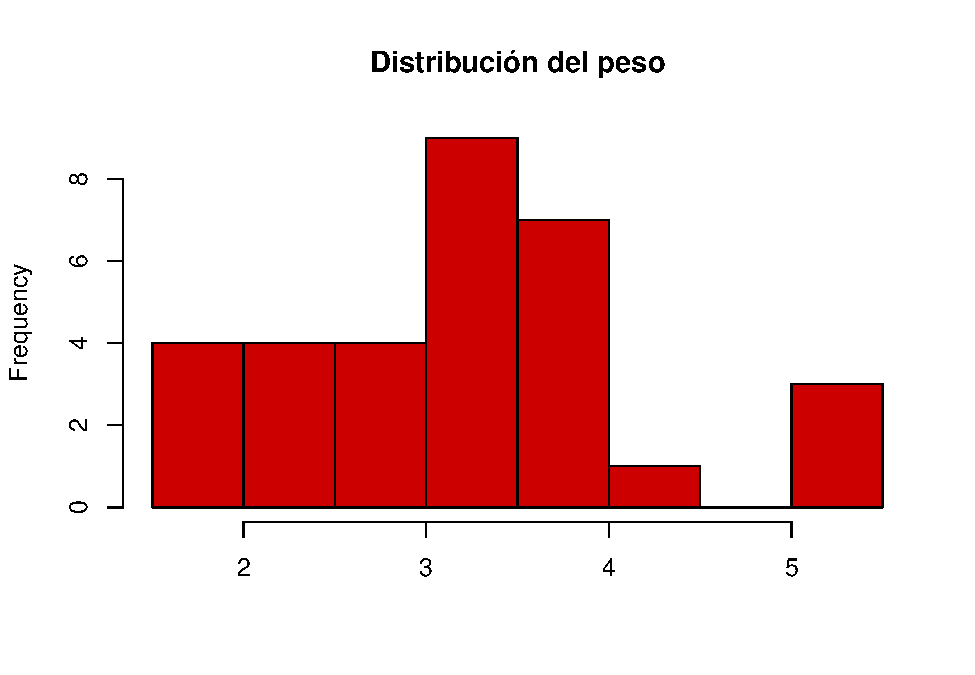
\includegraphics{Taller-R-1_files/figure-latex/unnamed-chunk-6-1.pdf}

\begin{Shaded}
\begin{Highlighting}[]
\FunctionTok{boxplot}\NormalTok{(d}\SpecialCharTok{$}\NormalTok{wt, }\AttributeTok{ylab =} \StringTok{\textquotesingle{}Peso (en miles)\textquotesingle{}}\NormalTok{)}
\end{Highlighting}
\end{Shaded}

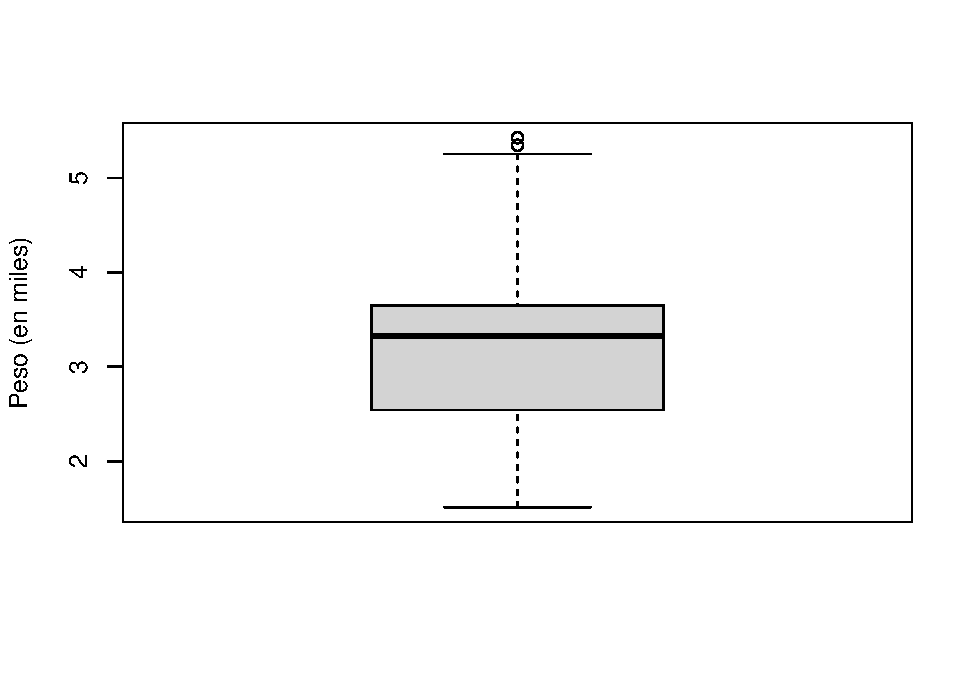
\includegraphics{Taller-R-1_files/figure-latex/unnamed-chunk-6-2.pdf}

\begin{Shaded}
\begin{Highlighting}[]
\FunctionTok{plot}\NormalTok{(d}\SpecialCharTok{$}\NormalTok{wt}\SpecialCharTok{\textasciitilde{}}\NormalTok{d}\SpecialCharTok{$}\NormalTok{mpg,}\AttributeTok{xlab=}\StringTok{"Millas por galón"}\NormalTok{,}\AttributeTok{ylab=}\StringTok{\textquotesingle{}Peso (en miles)\textquotesingle{}}\NormalTok{)}
\end{Highlighting}
\end{Shaded}

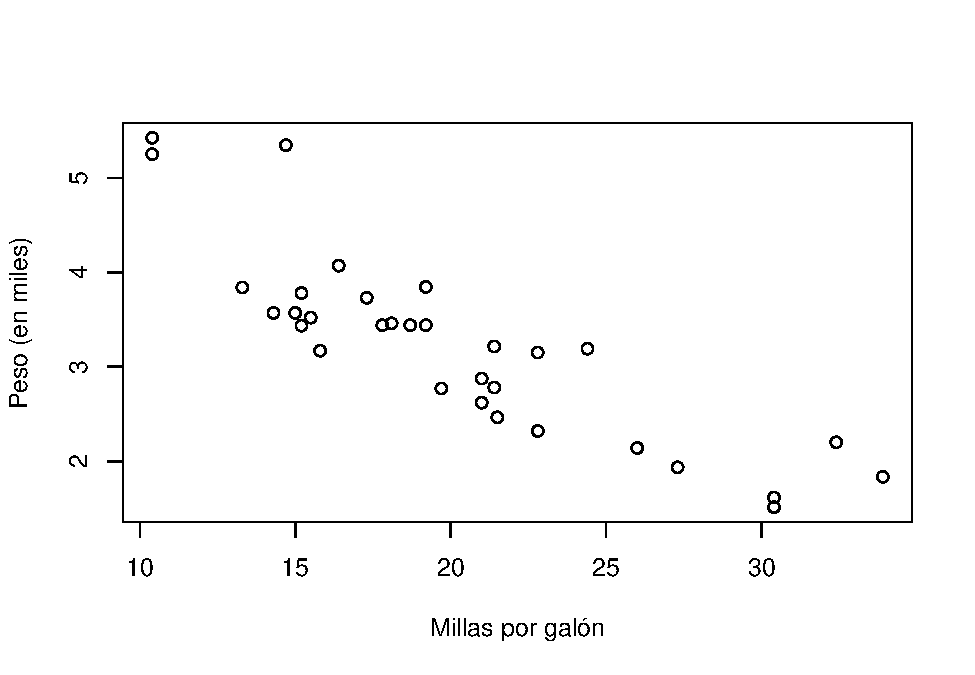
\includegraphics{Taller-R-1_files/figure-latex/unnamed-chunk-6-3.pdf}

Nota que para estas funciones lo que se \emph{requiere} en realidad es
el nombre de la variable como argumento. ¿Qué creen signifiquen las
opciones \texttt{col\ =}, \texttt{xlab\ =}, \texttt{main\ =}, y
\texttt{ylab\ =}?

Podríamos también agrupar la información como ocurre en estos casos
abajo del paquete \texttt{psych}.

\begin{Shaded}
\begin{Highlighting}[]
\CommentTok{\#install.packages("psych")}
\FunctionTok{library}\NormalTok{(psych)}
\end{Highlighting}
\end{Shaded}

\begin{verbatim}
## 
## Attaching package: 'psych'
\end{verbatim}

\begin{verbatim}
## The following objects are masked from 'package:ggplot2':
## 
##     %+%, alpha
\end{verbatim}

\begin{Shaded}
\begin{Highlighting}[]
\FunctionTok{describe}\NormalTok{(d}\SpecialCharTok{$}\NormalTok{hp) }\CommentTok{\# la función "describe" viene en el paquete de psych; da datos adicionales}
\end{Highlighting}
\end{Shaded}

\begin{verbatim}
##    vars  n   mean    sd median trimmed  mad min max range skew kurtosis    se
## X1    1 32 146.69 68.56    123  141.19 77.1  52 335   283 0.73    -0.14 12.12
\end{verbatim}

\begin{Shaded}
\begin{Highlighting}[]
\FunctionTok{describeBy}\NormalTok{(d}\SpecialCharTok{$}\NormalTok{mpg, d}\SpecialCharTok{$}\NormalTok{am) }\CommentTok{\# del paquete "psych"}
\end{Highlighting}
\end{Shaded}

\begin{verbatim}
## 
##  Descriptive statistics by group 
## group: 0
##    vars  n  mean   sd median trimmed  mad  min  max range skew kurtosis   se
## X1    1 19 17.15 3.83   17.3   17.12 3.11 10.4 24.4    14 0.01     -0.8 0.88
## ------------------------------------------------------------ 
## group: 1
##    vars  n  mean   sd median trimmed  mad min  max range skew kurtosis   se
## X1    1 13 24.39 6.17   22.8   24.38 6.67  15 33.9  18.9 0.05    -1.46 1.71
\end{verbatim}

Una forma más complicada pero útil de verificar estadísticas es la
función \texttt{xtabs()}, es decir tabulación cruzada. El código pide
una fórmula que contraste las variables. El código es un poco más
complicado pero se puede interpretar como ``la suma de \texttt{mpg},
para cada grupo de \texttt{cyl} y \texttt{am}''. Ya que \texttt{cyl}
tiene tres grupos y \texttt{am} tiene dos grupos, \texttt{xtabs()}
devuelve una tabla de seis celdas con las sumas de \texttt{mpg} para
cada uno de estos grupos; así podríamos por ejemplo verificar como
cambian las medias dadas ciertas categorías. Noten que hemos usado, sin
\texttt{attach()} el nombre de las variables, ya que le dijimos a la
función que se enfocara en las variables dentro del objeto definido en
la opción \texttt{data\ =\ conjunto\_de\_datos} (aquí, \emph{data} = d).

\begin{Shaded}
\begin{Highlighting}[]
\FunctionTok{xtabs}\NormalTok{(mpg }\SpecialCharTok{\textasciitilde{}}\NormalTok{ cyl }\SpecialCharTok{+}\NormalTok{ am, }\AttributeTok{data =}\NormalTok{ d)}
\end{Highlighting}
\end{Shaded}

\begin{verbatim}
##    am
## cyl     0     1
##   4  68.7 224.6
##   6  76.5  61.7
##   8 180.6  30.8
\end{verbatim}

Si queríamos el promedio de millas por galón por categoría hacemos lo
siguiente:

\begin{Shaded}
\begin{Highlighting}[]
\CommentTok{\# Sumamos mpg por categorías de cyl y am}
\NormalTok{suma\_mpg }\OtherTok{\textless{}{-}} \FunctionTok{xtabs}\NormalTok{(mpg }\SpecialCharTok{\textasciitilde{}}\NormalTok{ cyl }\SpecialCharTok{+}\NormalTok{ am, }\AttributeTok{data =}\NormalTok{ d)}

\CommentTok{\# Sacamos la cantidad de observaciones por categorías de cyl y am obviando el lado izquierdo de la fórmula}
\NormalTok{cantidad }\OtherTok{\textless{}{-}} \FunctionTok{xtabs}\NormalTok{(}\SpecialCharTok{\textasciitilde{}}\NormalTok{ cyl }\SpecialCharTok{+}\NormalTok{ am, }\AttributeTok{data =}\NormalTok{ d)}

\CommentTok{\# Media de mpg por categorías de cyl y am}
\NormalTok{media\_mpg }\OtherTok{\textless{}{-}}\NormalTok{ suma\_mpg }\SpecialCharTok{/}\NormalTok{ cantidad}

\NormalTok{media\_mpg}
\end{Highlighting}
\end{Shaded}

\begin{verbatim}
##    am
## cyl        0        1
##   4 22.90000 28.07500
##   6 19.12500 20.56667
##   8 15.05000 15.40000
\end{verbatim}

En este caso hemos obtenido la media de millas por galón según la
cantidad de cilindros del vehículo, y si la transmisión era manual o
automática.

\section{Entendiendo y manipulando datos:
Tidyverse}\label{entendiendo-y-manipulando-datos-tidyverse}

Si bien podríamos usar esta información previa para entender los datos.
Digamos que queremos saber qué carro es el mejor en estos datos en
cuestión de millas por galón. Podríamos hacer:

\begin{Shaded}
\begin{Highlighting}[]
\FunctionTok{library}\NormalTok{(ggplot2)}
\FunctionTok{data}\NormalTok{(}\StringTok{"mpg"}\NormalTok{)}
\FunctionTok{summary}\NormalTok{(mpg)}
\end{Highlighting}
\end{Shaded}

\begin{verbatim}
##  manufacturer          model               displ            year     
##  Length:234         Length:234         Min.   :1.600   Min.   :1999  
##  Class :character   Class :character   1st Qu.:2.400   1st Qu.:1999  
##  Mode  :character   Mode  :character   Median :3.300   Median :2004  
##                                        Mean   :3.472   Mean   :2004  
##                                        3rd Qu.:4.600   3rd Qu.:2008  
##                                        Max.   :7.000   Max.   :2008  
##       cyl           trans               drv                 cty       
##  Min.   :4.000   Length:234         Length:234         Min.   : 9.00  
##  1st Qu.:4.000   Class :character   Class :character   1st Qu.:14.00  
##  Median :6.000   Mode  :character   Mode  :character   Median :17.00  
##  Mean   :5.889                                         Mean   :16.86  
##  3rd Qu.:8.000                                         3rd Qu.:19.00  
##  Max.   :8.000                                         Max.   :35.00  
##       hwy             fl               class          
##  Min.   :12.00   Length:234         Length:234        
##  1st Qu.:18.00   Class :character   Class :character  
##  Median :24.00   Mode  :character   Mode  :character  
##  Mean   :23.44                                        
##  3rd Qu.:27.00                                        
##  Max.   :44.00
\end{verbatim}

\begin{Shaded}
\begin{Highlighting}[]
\FunctionTok{max}\NormalTok{(mpg}\SpecialCharTok{$}\NormalTok{hwy) }\CommentTok{\#sin embargo esto no nos lleva a mucha más información}
\end{Highlighting}
\end{Shaded}

\begin{verbatim}
## [1] 44
\end{verbatim}

\begin{Shaded}
\begin{Highlighting}[]
\NormalTok{i\_max}\OtherTok{\textless{}{-}}\FunctionTok{which.max}\NormalTok{(mpg}\SpecialCharTok{$}\NormalTok{hwy)}
\NormalTok{mpg}\SpecialCharTok{$}\NormalTok{model[i\_max]}
\end{Highlighting}
\end{Shaded}

\begin{verbatim}
## [1] "jetta"
\end{verbatim}

El vehículo con mejor millaje por galón fue el Jetta. Igualmente si
trabajamos datos de criminalidad en EEUU, podríamos tener

\begin{Shaded}
\begin{Highlighting}[]
\FunctionTok{library}\NormalTok{(dslabs)}
\FunctionTok{data}\NormalTok{(murders)}
\FunctionTok{summary}\NormalTok{(murders)}
\end{Highlighting}
\end{Shaded}

\begin{verbatim}
##     state               abb                      region     population      
##  Length:51          Length:51          Northeast    : 9   Min.   :  563626  
##  Class :character   Class :character   South        :17   1st Qu.: 1696962  
##  Mode  :character   Mode  :character   North Central:12   Median : 4339367  
##                                        West         :13   Mean   : 6075769  
##                                                           3rd Qu.: 6636084  
##                                                           Max.   :37253956  
##      total       
##  Min.   :   2.0  
##  1st Qu.:  24.5  
##  Median :  97.0  
##  Mean   : 184.4  
##  3rd Qu.: 268.0  
##  Max.   :1257.0
\end{verbatim}

\begin{Shaded}
\begin{Highlighting}[]
\FunctionTok{min}\NormalTok{(murders}\SpecialCharTok{$}\NormalTok{total) }\CommentTok{\#queremos igual aquí saber el estado que menos tuvo}
\end{Highlighting}
\end{Shaded}

\begin{verbatim}
## [1] 2
\end{verbatim}

\begin{Shaded}
\begin{Highlighting}[]
\NormalTok{i\_min}\OtherTok{\textless{}{-}}\FunctionTok{which.min}\NormalTok{(murders}\SpecialCharTok{$}\NormalTok{total)}
\NormalTok{murders}\SpecialCharTok{$}\NormalTok{state[i\_min]}
\end{Highlighting}
\end{Shaded}

\begin{verbatim}
## [1] "Vermont"
\end{verbatim}

Y tendríamos este resultado, con Vermont como el que menos asesinatos de
arma de fuego registrara en 2010.

Sin embargo esto no es suficiente quizás para todo lo que queremos hacer
y se ve demasiado laborioso o largo en relación a lo que obtenemos. En
el caso de los datos de asesinatos por arma de fuego, hemos buscado el
estado con menos asesinatos, y vemos que hay un rango enorme entre ése y
el mayor, pero ¿estamos comparando chinas con chinas?

\subsection{Modificando conjuntos de datos: creando una
variable}\label{modificando-conjuntos-de-datos-creando-una-variable}

Podríamos crear una tasa de asesinatos para este último conjunto de
datos, con la información ya suministrada.

\begin{Shaded}
\begin{Highlighting}[]
\NormalTok{murders}\SpecialCharTok{$}\NormalTok{tasa\_100k}\OtherTok{\textless{}{-}}\NormalTok{murders}\SpecialCharTok{$}\NormalTok{total}\SpecialCharTok{/}\NormalTok{murders}\SpecialCharTok{$}\NormalTok{population }\SpecialCharTok{*}\DecValTok{10}\SpecialCharTok{\^{}}\DecValTok{5}
\FunctionTok{head}\NormalTok{(murders)}
\end{Highlighting}
\end{Shaded}

\begin{verbatim}
##        state abb region population total tasa_100k
## 1    Alabama  AL  South    4779736   135  2.824424
## 2     Alaska  AK   West     710231    19  2.675186
## 3    Arizona  AZ   West    6392017   232  3.629527
## 4   Arkansas  AR  South    2915918    93  3.189390
## 5 California  CA   West   37253956  1257  3.374138
## 6   Colorado  CO   West    5029196    65  1.292453
\end{verbatim}

\begin{Shaded}
\begin{Highlighting}[]
\CommentTok{\#en tidyverse esto se puede hacer con la función mutate()}
\NormalTok{murders}\OtherTok{\textless{}{-}}\FunctionTok{mutate}\NormalTok{(murders,}\AttributeTok{tasa=}\NormalTok{total}\SpecialCharTok{/}\NormalTok{population}\SpecialCharTok{*}\DecValTok{10}\SpecialCharTok{\^{}}\DecValTok{5}\NormalTok{)}
\FunctionTok{head}\NormalTok{(murders)}
\end{Highlighting}
\end{Shaded}

\begin{verbatim}
##        state abb region population total tasa_100k     tasa
## 1    Alabama  AL  South    4779736   135  2.824424 2.824424
## 2     Alaska  AK   West     710231    19  2.675186 2.675186
## 3    Arizona  AZ   West    6392017   232  3.629527 3.629527
## 4   Arkansas  AR  South    2915918    93  3.189390 3.189390
## 5 California  CA   West   37253956  1257  3.374138 3.374138
## 6   Colorado  CO   West    5029196    65  1.292453 1.292453
\end{verbatim}

Digamos que ahora queremos ver una lista más informativa e intuitiva de
los datos; por ejemplo, qué otros carros figuran con buen millaje por
galón:

\begin{Shaded}
\begin{Highlighting}[]
\FunctionTok{filter}\NormalTok{(mpg, hwy}\SpecialCharTok{\textgreater{}=}\DecValTok{35}\NormalTok{) }
\end{Highlighting}
\end{Shaded}

\begin{verbatim}
## # A tibble: 8 x 11
##   manufacturer model      displ  year   cyl trans  drv     cty   hwy fl    class
##   <chr>        <chr>      <dbl> <int> <int> <chr>  <chr> <int> <int> <chr> <chr>
## 1 honda        civic        1.8  2008     4 auto(~ f        25    36 r     subc~
## 2 honda        civic        1.8  2008     4 auto(~ f        24    36 c     subc~
## 3 toyota       corolla      1.8  1999     4 manua~ f        26    35 r     comp~
## 4 toyota       corolla      1.8  2008     4 manua~ f        28    37 r     comp~
## 5 toyota       corolla      1.8  2008     4 auto(~ f        26    35 r     comp~
## 6 volkswagen   jetta        1.9  1999     4 manua~ f        33    44 d     comp~
## 7 volkswagen   new beetle   1.9  1999     4 manua~ f        35    44 d     subc~
## 8 volkswagen   new beetle   1.9  1999     4 auto(~ f        29    41 d     subc~
\end{verbatim}

En este caso hemos seleccionado las filas para visualizar que tienen
millaje por galón superior a 35: hemos creado un \textbf{subconjunto}.

\subsection{\texorpdfstring{El operador pipe \texttt{\%\textgreater{}\%}
o
\texttt{\textbar{}\textgreater{}}}{El operador pipe \%\textgreater\% o \textbar\textgreater{}}}\label{el-operador-pipe-o}

Digamos que realmente queremos reducir la cantidad de columnas en las
que queremos enfocarnos, pues los datos de \texttt{mpg} tienen
demasiadas. Podríamos crear otro subconjunto:

\begin{Shaded}
\begin{Highlighting}[]
\NormalTok{tabla\_nueva\_mpg}\OtherTok{\textless{}{-}}\FunctionTok{select}\NormalTok{(mpg,model,year,cty,hwy)}
\FunctionTok{filter}\NormalTok{(tabla\_nueva\_mpg, hwy}\SpecialCharTok{\textgreater{}=}\DecValTok{35}\NormalTok{) }
\end{Highlighting}
\end{Shaded}

\begin{verbatim}
## # A tibble: 8 x 4
##   model       year   cty   hwy
##   <chr>      <int> <int> <int>
## 1 civic       2008    25    36
## 2 civic       2008    24    36
## 3 corolla     1999    26    35
## 4 corolla     2008    28    37
## 5 corolla     2008    26    35
## 6 jetta       1999    33    44
## 7 new beetle  1999    35    44
## 8 new beetle  1999    29    41
\end{verbatim}

Y nos quedamos con cuatro columnas dándonos información puntual si esto
era lo que nos interesaba. Sin embargo, podríamos evitarnos la creación
de objetos intermedios al usar la función que canaliza los datos en
secuencia funcional así:

\begin{Shaded}
\begin{Highlighting}[]
\NormalTok{mpg }\SpecialCharTok{\%\textgreater{}\%} \FunctionTok{select}\NormalTok{(model,year,cty,hwy) }\SpecialCharTok{|\textgreater{}} \FunctionTok{filter}\NormalTok{(hwy}\SpecialCharTok{\textgreater{}=}\DecValTok{35}\NormalTok{)}
\end{Highlighting}
\end{Shaded}

\begin{verbatim}
## # A tibble: 8 x 4
##   model       year   cty   hwy
##   <chr>      <int> <int> <int>
## 1 civic       2008    25    36
## 2 civic       2008    24    36
## 3 corolla     1999    26    35
## 4 corolla     2008    28    37
## 5 corolla     2008    26    35
## 6 jetta       1999    33    44
## 7 new beetle  1999    35    44
## 8 new beetle  1999    29    41
\end{verbatim}

\emph{Vale la pena señalar que el} pipe \emph{funcionará bien con las
funciones donde el primer argumento sean los datos de entrada, que
canalizamos. Las funciones de tidyr y dplyr operan así y se acoplan al}
pipe\emph{.}

\subsection{Resumiendo datos explorativamente con
Tidy}\label{resumiendo-datos-explorativamente-con-tidy}

En esta sección cubriremos dos funciones de tidyverse, en dplyr,
\texttt{summarise} y \texttt{group\_by}. La primera, \texttt{summarise},
ofrece el cálculo de estadísticas de resumen con un código legible e
intuitivo. El segundo agrupa y resume los datos por categorías inherente
en las variables existentes. Por ejemplo, quizás quisiéramos calcular el
promedio y desviación estándar de los vehículos en los datos de millaje
por galón, pero queremos agruparlos por fabricante, o tipo de
transmisión, o cualquier otro tipo de variable:

\begin{Shaded}
\begin{Highlighting}[]
\NormalTok{mpg }\SpecialCharTok{\%\textgreater{}\%}
  \FunctionTok{group\_by}\NormalTok{(manufacturer) }\SpecialCharTok{|\textgreater{}}
  \FunctionTok{summarise}\NormalTok{(}\AttributeTok{mpg\_grupal=}\FunctionTok{mean}\NormalTok{(hwy),}
            \AttributeTok{ds\_grupal=}\FunctionTok{sd}\NormalTok{(hwy)) }\CommentTok{\#por fabricador}
\end{Highlighting}
\end{Shaded}

\begin{verbatim}
## # A tibble: 15 x 3
##    manufacturer mpg_grupal ds_grupal
##    <chr>             <dbl>     <dbl>
##  1 audi               26.4      2.18
##  2 chevrolet          21.9      5.11
##  3 dodge              17.9      3.57
##  4 ford               19.4      3.33
##  5 honda              32.6      2.55
##  6 hyundai            26.9      2.18
##  7 jeep               17.6      3.25
##  8 land rover         16.5      1.73
##  9 lincoln            17        1   
## 10 mercury            18        1.15
## 11 nissan             24.6      5.09
## 12 pontiac            26.4      1.14
## 13 subaru             25.6      1.16
## 14 toyota             24.9      6.17
## 15 volkswagen         29.2      5.32
\end{verbatim}

\begin{Shaded}
\begin{Highlighting}[]
\NormalTok{mpg }\SpecialCharTok{|\textgreater{}}
  \FunctionTok{group\_by}\NormalTok{(trans) }\SpecialCharTok{|\textgreater{}}
  \FunctionTok{summarise}\NormalTok{(}\AttributeTok{mpg\_grupal=}\FunctionTok{mean}\NormalTok{(hwy),}
            \AttributeTok{ds\_grupal=}\FunctionTok{sd}\NormalTok{(hwy)) }\CommentTok{\#por año de manufactura}
\end{Highlighting}
\end{Shaded}

\begin{verbatim}
## # A tibble: 10 x 3
##    trans      mpg_grupal ds_grupal
##    <chr>           <dbl>     <dbl>
##  1 auto(av)         27.8      2.59
##  2 auto(l3)         27        4.24
##  3 auto(l4)         22.0      5.64
##  4 auto(l5)         20.7      6.04
##  5 auto(l6)         20        2.37
##  6 auto(s4)         25.7      1.15
##  7 auto(s5)         25.3      6.66
##  8 auto(s6)         25.2      3.99
##  9 manual(m5)       26.3      5.99
## 10 manual(m6)       24.2      5.75
\end{verbatim}

Podemos también aplicar una función creada previamente:

\begin{Shaded}
\begin{Highlighting}[]
\NormalTok{mpg }\SpecialCharTok{|\textgreater{}} \FunctionTok{group\_by}\NormalTok{(manufacturer) }\SpecialCharTok{|\textgreater{}} \FunctionTok{summarise}\NormalTok{(mediana\_mín\_máx(hwy))}
\end{Highlighting}
\end{Shaded}

\begin{verbatim}
## # A tibble: 15 x 4
##    manufacturer mediana   mín   máx
##    <chr>          <dbl> <dbl> <dbl>
##  1 audi            26      23    31
##  2 chevrolet       23      14    30
##  3 dodge           17      12    24
##  4 ford            18      15    26
##  5 honda           32      29    36
##  6 hyundai         26.5    24    31
##  7 jeep            18.5    12    22
##  8 land rover      16.5    15    18
##  9 lincoln         17      16    18
## 10 mercury         18      17    19
## 11 nissan          26      17    32
## 12 pontiac         26      25    28
## 13 subaru          26      23    27
## 14 toyota          26      15    37
## 15 volkswagen      29      23    44
\end{verbatim}

Digamos que queremos obtener las tasas medias de regiones específicas en
los EEUU. En este caso entra más complicación pero en Tidyverse podemos
usar tanto el pipe \texttt{\%\textgreater{}\%} como la \texttt{\%in\%}
(el \%in\% es una función que busca parear la entrada de un valor
mapeado en otro):

\begin{Shaded}
\begin{Highlighting}[]
\NormalTok{murders }\SpecialCharTok{\%\textgreater{}\%}
  \FunctionTok{mutate}\NormalTok{(}\AttributeTok{group =} \FunctionTok{case\_when}\NormalTok{(}
\NormalTok{    abb }\SpecialCharTok{\%in\%} \FunctionTok{c}\NormalTok{(}\StringTok{"ME"}\NormalTok{, }\StringTok{"NH"}\NormalTok{, }\StringTok{"VT"}\NormalTok{, }\StringTok{"MA"}\NormalTok{, }\StringTok{"RI"}\NormalTok{, }\StringTok{"CT"}\NormalTok{) }\SpecialCharTok{\textasciitilde{}} \StringTok{"Nueva Inglaterra"}\NormalTok{,}
\NormalTok{    abb }\SpecialCharTok{\%in\%} \FunctionTok{c}\NormalTok{(}\StringTok{"WA"}\NormalTok{, }\StringTok{"OR"}\NormalTok{, }\StringTok{"CA"}\NormalTok{) }\SpecialCharTok{\textasciitilde{}} \StringTok{"Costa del Pacífico"}\NormalTok{,}
\NormalTok{    region }\SpecialCharTok{==} \StringTok{"South"} \SpecialCharTok{\textasciitilde{}} \StringTok{"el Sur"}\NormalTok{,}
    \ConstantTok{TRUE} \SpecialCharTok{\textasciitilde{}} \StringTok{"Otras regiones"}\NormalTok{)) }\SpecialCharTok{\%\textgreater{}\%}
  \FunctionTok{group\_by}\NormalTok{(group) }\SpecialCharTok{\%\textgreater{}\%}
  \FunctionTok{summarise}\NormalTok{(}\AttributeTok{tasa\_100k =} \FunctionTok{sum}\NormalTok{(total)}\SpecialCharTok{/} \FunctionTok{sum}\NormalTok{(population) }\SpecialCharTok{*} \DecValTok{10}\SpecialCharTok{\^{}}\DecValTok{5}\NormalTok{)}
\end{Highlighting}
\end{Shaded}

\begin{verbatim}
## # A tibble: 4 x 2
##   group              tasa_100k
##   <chr>                  <dbl>
## 1 Costa del Pacífico      2.90
## 2 Nueva Inglaterra        1.72
## 3 Otras regiones          2.71
## 4 el Sur                  3.63
\end{verbatim}

\section{Recapitulando}\label{recapitulando}

\subsection{Qué aprendimos en este taller
inicial}\label{quuxe9-aprendimos-en-este-taller-inicial}

Hoy aprendimos varias cosas para empezar a usar R:

\begin{itemize}
\tightlist
\item
  Hablamos sobre cómo descargar e instalar R y RStudio;
\item
  Funcionalidades posibles, como Markdown;
\item
  Funciones y jerga específica de R;
\item
  Cómo cargar datos y visualizarlos;
\item
  Cómo buscar estadísticas básicas;
\item
  Cómo llevar a cabo operaciones transformadoras a los datos;
\item
  Empezamos a usar la sintaxis de tidyverse.
\end{itemize}

\subsection{Continuamos el próximo
miércoles}\label{continuamos-el-pruxf3ximo-miuxe9rcoles}

En los talleres que vienen continuaremos ahondando en operaciones
estadísticas, visualización más avanzada, estadística inferencial y
análisis de redes. Gracias por asistir hoy.

\end{document}
